% Chapter 6

\chapter{Problems}
\label{Chapter6} 
By identifying  the requirements, we could then be able to highlight the related problems that we had to face in order to fulfill all of them. We will describe the related requirement as source of each faced problem.

\section{Mobile platform fragmentation}
Considering the requirement of a wide platform compatibility, we obviously need to face a really big problem in the mobile application world: the platform fragmentation.\\
Starting from the first smartphone release on 2007, the iPhone from Apple,  the sale of such devices keeps increasing each year. Between 2007 and 2008 sales proceeded upwards reaching the same sale rate of their computing parent, the PC. On 2009  the market signed an important inflection point, representing the beginning of an inexorable vertical rise. Although PCs were still the only ones to offer some types of functionality due to their longer replacement cycle, they were sold with a ratio of 1 : 2, compared to smartphones, over a 5 year period. This new market’ growth leads to an obvious seeking of various participants, some by choice and some by necessity, in order to extract value. Android has been the prime beneficiary, having been announced on 2007 and having gone on to account for well over half of smartphone sales worldwide. Apple, meanwhile, has maintained a steady ship, leveraging its skill in product design and user experience with a finely honed marketing machine, attracting a customer that rarely defects.\cite{ref5}
\begin{figure}[ht!]
	\centering
	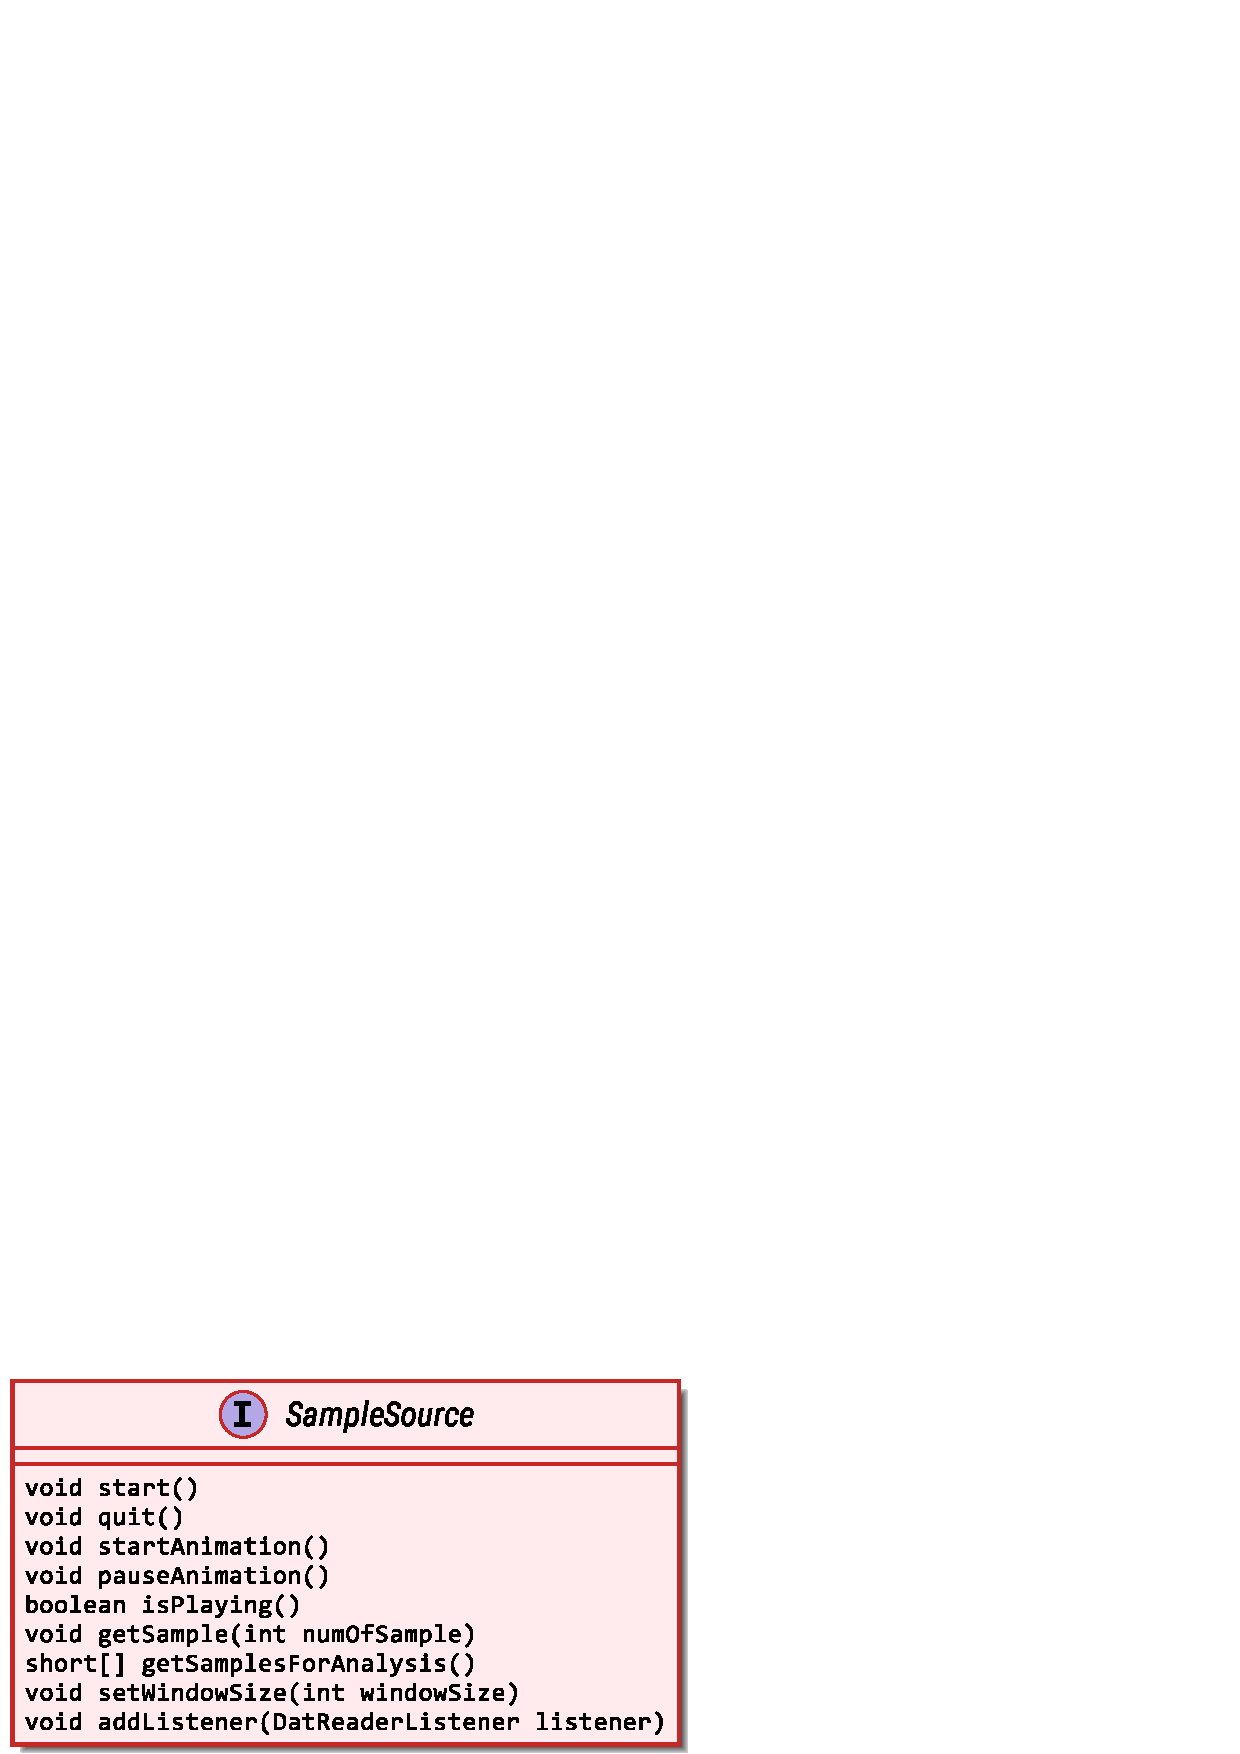
\includegraphics[width=120mm]{figures/ch6/1.png}
	\caption{Mobile platform share evolution (smartphone sales), 2009–13.}
	\label{fig6.1}
\end{figure}
Fast-forwarding to 2016, if we consider the global market share held by the leading smartphone operating systems, at first position we have Android with a share of  80.7\%, followed by iOS with a 17.7\%. Minor percentages are represented by Windows Phone (1.1\%), RIM (0.2\%) and others (0.2\%).\cite{ref6}

\section{Native vs Cross-Platform}
As mentioned earlier, one of the main challenges when moving to a mobile solution is the software development within a technology landscape that is highly fragmented and rapidly evolving. Mobile apps require a fair amount of customization to run on diverse platforms and a constant update due to the steady stream of new hardware, OS versions and browsers. Even a single platform (Android, Windows, Blackberry, and to a lesser extent Apple) has numerous flavors that require some degree of customization. There are also other factors such as the overlay software from different manufacturers that can affect behavior of an app on a particular device.\\
In response, the mobile industry has spawned a rapidly growing ecosystem of cross-platform and cross-device frameworks, source code analyzers, libraries of reusable components, and other tools designed to accelerate and simplify multi-platform development. New tools are constantly emerging, with new functionality, different capabilities,  strengths and weaknesses.\\
Developer’s preferences change and evolve, particularly as new tools and capabilities become available. However, the basic goals are the same: to code less and accomplish more, to reuse and recycle across multiple platforms as much as possible, and consider developing from scratch as the last resort. In addition, any tool or framework should be able to work with current and future evolving offers, and not to be locked because of a particular platform or technology.\cite{ref7}
